\documentclass[10pt]{article}

\usepackage[T1]{fontenc}
\usepackage[utf8]{inputenc}
\usepackage{lmodern}
\usepackage[margin=0.82in]{geometry}
\usepackage{amsmath,amssymb}
\usepackage{booktabs,tabularx,array,longtable}
\usepackage{graphicx}
\usepackage{float}
\usepackage{xspace}
\usepackage{xcolor}
\usepackage{tikz}
\usetikzlibrary{arrows.meta,positioning,shapes.geometric}
\usepackage[numbers,sort&compress]{natbib}
\usepackage{url}
\usepackage[colorlinks=true,allcolors=teal!55!black]{hyperref}
\emergencystretch=2em

\definecolor{ink}{HTML}{17323A}
\definecolor{muted}{HTML}{51666B}
\definecolor{orange}{HTML}{D68155}
\definecolor{tealpaper}{HTML}{398783}
\definecolor{redpaper}{HTML}{A54132}
\newcolumntype{Y}{>{\raggedright\arraybackslash}X}
\newcommand{\Base}{\textsc{Base}\xspace}
\newcommand{\Detour}{\textsc{Detour}\xspace}
\newcommand{\Retreat}{\textsc{Retreat}\xspace}
\newcommand{\Oracle}{\textsc{Oracle}\xspace}
\newcommand{\RiskBest}{\textsc{Risk}$\rightarrow$\textsc{BestFixed}\xspace}
\newcommand{\source}{\texttt{source\_state\_sha256}\xspace}
\graphicspath{{../../../results/iclr27/risk_value_decoupling_dc48ff317dad_20260829T154351Z/}}

\title{\textbf{Risk Does Not Specify Intervention: Exact-State Diagnostics for an OpenVLA--LIBERO Safety Case Study}}
\author{Anonymous authors}
\date{}

\begin{document}
\maketitle

\begin{abstract}
Runtime safety for vision-language-action policies is often formulated as
predicting whether nominal behavior will catastrophize. That binary label does
not identify whether intervention improves realized utility, which finite
option is best, or whether a statewise opportunity can be reached
sequentially. We study these distinctions in one frozen OpenVLA--LIBERO
\texttt{glass\_recovery} exact-state design. From identical hash-verified
branch starts, we execute \Base, a privileged task-preserving \Detour, and a
conservative \Retreat under a common task-success, catastrophe, and safe-
noncompletion utility. All 20 sources and 273 eligible decisions are exposed
development evidence. Binary Base risk and intervention benefit disagree on
19/273 decisions across 12 sources. Exhaustive tight matching yields three
same-risk, different-strict-action pairs across two sources; the exact
\Detour--\Retreat witness has only one independent source. Source-macro utility
is 0.2544 for \RiskBest and 0.5642 for the realized finite-option \Oracle,
leaving an observed opportunity of 0.3097. The strongest evaluated
OutcomeRouter gains only +0.0178 over \RiskBest and no method gate passes; the
full tiny advantage-decomposed router reaches only 0.2311. Support is
mechanically concentrated: all 23 strict \Retreat states and 51/60 strict
\Detour-or-\Retreat states are glass. At fresh sequential first crossing, the
direct selector chooses \Base on 24/24 episodes, recovers 0/8 glass episodes,
and misses 2/2 known opportunities. The result is therefore a glass-scoped
exact-state diagnostic and negative-result case study, not a successful router
or a broad VLA-safety benchmark.
\end{abstract}

\section{Introduction}

Consider two saved states from the same source, the same glass condition, the
same five-action horizon, and the same binary observation that continuing
\Base catastrophizes. In state \texttt{43347d99...}, realized outcomes for
(\Base, \Detour, \Retreat) are (catastrophe, task success, safe
noncompletion), so \Detour is uniquely best. In state \texttt{f83d0199...},
the outcomes are (catastrophe, catastrophe, safe noncompletion), so \Retreat is
uniquely best. A perfect binary risk bit is identical for the pair but cannot
specify the action. This witness is deliberately narrow: both states come from
one source in one mechanical design. Its value is diagnostic, not universal.

This distinction matters whenever a runtime system can choose among preserving
the nominal policy, attempting task-preserving recovery, and stopping or
retreating safely. Failure detection asks whether nominal continuation is bad.
Intervention asks a different question: whether any available alternative is
better, and if so which one. A further gap separates a choice that is clear at
an authored saved state from one that a sequential policy can realize at the
right time. We write these four targets as
\[
  \text{Base risk}\;\neq\;\text{intervention benefit}
  \;\neq\;\text{best finite option}
  \;\neq\;\text{sequential realization}.
\]

We use the frozen CrashBench exact-state corpus to measure those distinctions
without introducing a new learned method or collecting another outcome. At
each eligible decision, three controllers are executed from the same verified
branch start. The resulting finite-option outcomes support a source-aware
diagnosis of risk-benefit disagreement, strict action ambiguity, policy
regret, and oracle-hybrid attribution. The strongest learned selectors remain
null under their frozen gates, and a fresh sequential evaluation collapses to
\Base. The appropriate scientific object is therefore the diagnostic protocol
and its scoped negative result.

Our contributions are exactly four:
\begin{enumerate}
  \item an exact-state realized-option protocol that restores a complete
  simulator/controller/continuation state and executes every member of a
  finite option set, observing outcomes instead of predicting them with a
  learned world model;
  \item a source-aware risk-regret diagnosis that separately measures Base
  risk, intervention benefit, strict option support, same-risk action
  ambiguity, and risk-only policy regret;
  \item a fair-baseline null and oracle attribution showing that the evaluated
  learned selectors do not pass the frozen method gate and that benefit gating
  accounts for most of the reported oracle-hybrid loss; and
  \item a statewise-to-sequential boundary preserving the fresh first-crossing
  null: statewise option opportunity does not imply reliable sequential
  realization.
\end{enumerate}

The evidence is one OpenVLA checkpoint, one LIBERO pick-and-place task, and one
\texttt{glass\_recovery} mechanical family. The labels \texttt{glass},
\texttt{offpath}, and \texttt{noglass} are a treatment and matched controls,
not three hazard families. We make no claim of a deployable router, broad
benchmark, cross-mechanism generality, or reliable sequential intervention.

\section{Related Work and Novelty Boundary}

\paragraph{VLA policies and failure detection.}
OpenVLA supplies the frozen policy and LIBERO supplies the manipulation
environment used in this case study \citep{kim2024openvla,liu2023libero}.
SAFE learns scalar failure scores from VLA internal features across tasks and
policies \citep{gu2025safe}; Hide-and-Seek localizes trajectory failure signals
from coarse labels \citep{park2026hide}. Our result is not a new failure
detector. It uses all realized outcomes of a fixed option set at identical
saved states to ask what a scalar failure target leaves unidentified.

\paragraph{Runtime verification and selective intervention.}
CheckVLA uses an action-conditioned world model to verify and rewrite action
suffixes \citep{liu2026checkvla}. CoWAM selects among shared candidate pools
using predicted futures and coordination contracts \citep{liu2026cowam}; this
is the nearest selective-intervention comparison. Model-based runtime
monitoring with interactive imitation learning anticipates failures and can
request oversight \citep{liu2023runtime}. CrashBench neither learns a rollout
world model nor proposes a deployment layer. Its narrower distinction is
realized, full-information branching for three fixed options from serialized
simulator states, followed by source-paired diagnosis. CheckVLA and the
monitoring literature have substantially broader sequential evidence.

\paragraph{Safety alignment, steering, and counterfactual language.}
SafeVLA changes the policy through constrained learning
\citep{zhang2025safevla}; our OpenVLA checkpoint remains frozen. Mechanistic
activation steering can causally change VLA behavior
\citep{haon2025steering}, so our historical final-readout steering null is not
a general statement about steerability. Counterfactual VLA generates reasoning
traces that revise driving meta-actions \citep{peng2025counterfactualvla}, while
counterfactual safe reinforcement learning constrains harm relative to a
default policy \citep{vaskov2024donoharm}. Here ``counterfactual'' means only
that each listed controller was actually executed from an identical saved
simulator state. We do not claim an observational causal estimator, language
self-reflection, or novelty from the term itself.

\section{Exact-State Realized-Option Protocol}
\label{sec:protocol}

\subsection{System, sources, and eligibility}

The frozen capture uses checkpoint revision \texttt{962318ce...c873} of the
OpenVLA LIBERO-Spatial checkpoint (full identity in
Appendix~\ref{app:provenance}). Decoding is deterministic
(no sampling, one beam), and the rollout seed is 0. The retained corpus has 20
unique \source values and 273 eligible decisions. Historical split labels are
5 train, 7 calibration, and 8 development sources, but they have all been
inspected and reused during the successive audits. We therefore treat all 20
as exposed development and make no confirmatory claim.

Each source contributes matched placements and conditions at remaining-action
horizons 40, 30, 20, 10, or 5 when mechanically eligible. Eligibility is
resolved before method comparison from Base and mechanical contracts. The
independent unit is the source state. Conditions, placements, horizons,
branches, and frames are repeated observations nested within a source.

\subsection{Branch and restoration contract}

Figure~\ref{fig:protocol-flow} summarizes the protocol. The collector rebuilds
the exact model XML, restores flattened MuJoCo time, position, and velocity
state, restores OSC/controller interpolation state, episode counters, robot
buffers, observable timing and cached observations, and restores the explicit
policy-boundary observation. Before every option, it requires equality of five
SHA-256 identities: simulator state, controller state, the full numeric
continuation snapshot, observation dictionary, and model XML. A mismatch
fails the decision rather than entering the corpus.

The capture also fixes the rollout seed and uses deterministic policy decoding
and deterministic structured controllers. It does not retain a separate
per-decision hash of global Python/NumPy/framework RNG bytes. We consequently
describe exact restoration at the five verified state boundaries above and do
not claim a stronger byte-level RNG restoration audit. This distinction is
recorded in the reproducibility statement and appendix.

\begin{figure}[H]
  \centering
  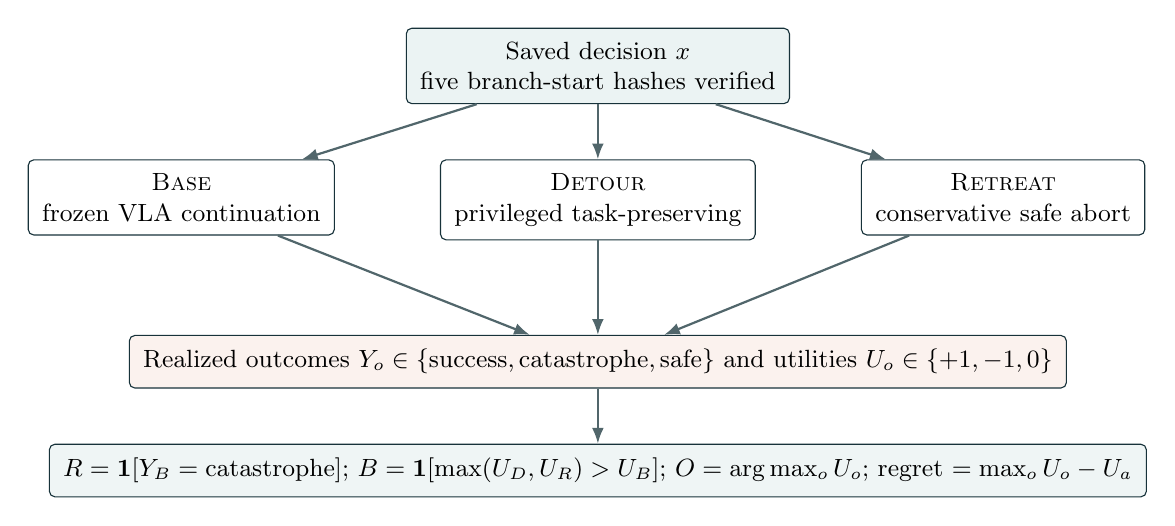
\begin{tikzpicture}[
      node distance=7mm and 9mm,
      box/.style={draw=ink, rounded corners=2pt, align=center, inner sep=5pt,
                  font=\small, fill=white},
      opt/.style={box, minimum width=32mm},
      arr/.style={-{Latex[length=2mm]}, thick, draw=muted}]
    \node[box, fill=tealpaper!10, minimum width=45mm] (state)
      {Saved decision $x$\\five branch-start hashes verified};
    \node[opt, below left=of state] (base) {\Base\\frozen VLA continuation};
    \node[opt, below=of state] (detour) {\Detour\\privileged task-preserving};
    \node[opt, below right=of state] (retreat) {\Retreat\\conservative safe abort};
    \draw[arr] (state) -- (base);
    \draw[arr] (state) -- (detour);
    \draw[arr] (state) -- (retreat);
    \node[box, below=12mm of detour, minimum width=100mm, fill=orange!10] (out)
      {Realized outcomes $Y_o\in\{\mathrm{success},\mathrm{catastrophe},\mathrm{safe}\}$ and utilities
       $U_o\in\{+1,-1,0\}$};
    \draw[arr] (base) -- (out);
    \draw[arr] (detour) -- (out);
    \draw[arr] (retreat) -- (out);
    \node[box, below=of out, minimum width=115mm, fill=tealpaper!8] (targets)
      {$R=\mathbf{1}[Y_B=\mathrm{catastrophe}]$; $B=\mathbf{1}[\max(U_D,U_R)>U_B]$;
       $O=\arg\max_o U_o$; regret $=\max_oU_o-U_a$};
    \draw[arr] (out) -- (targets);
  \end{tikzpicture}
  \vspace{3mm}

  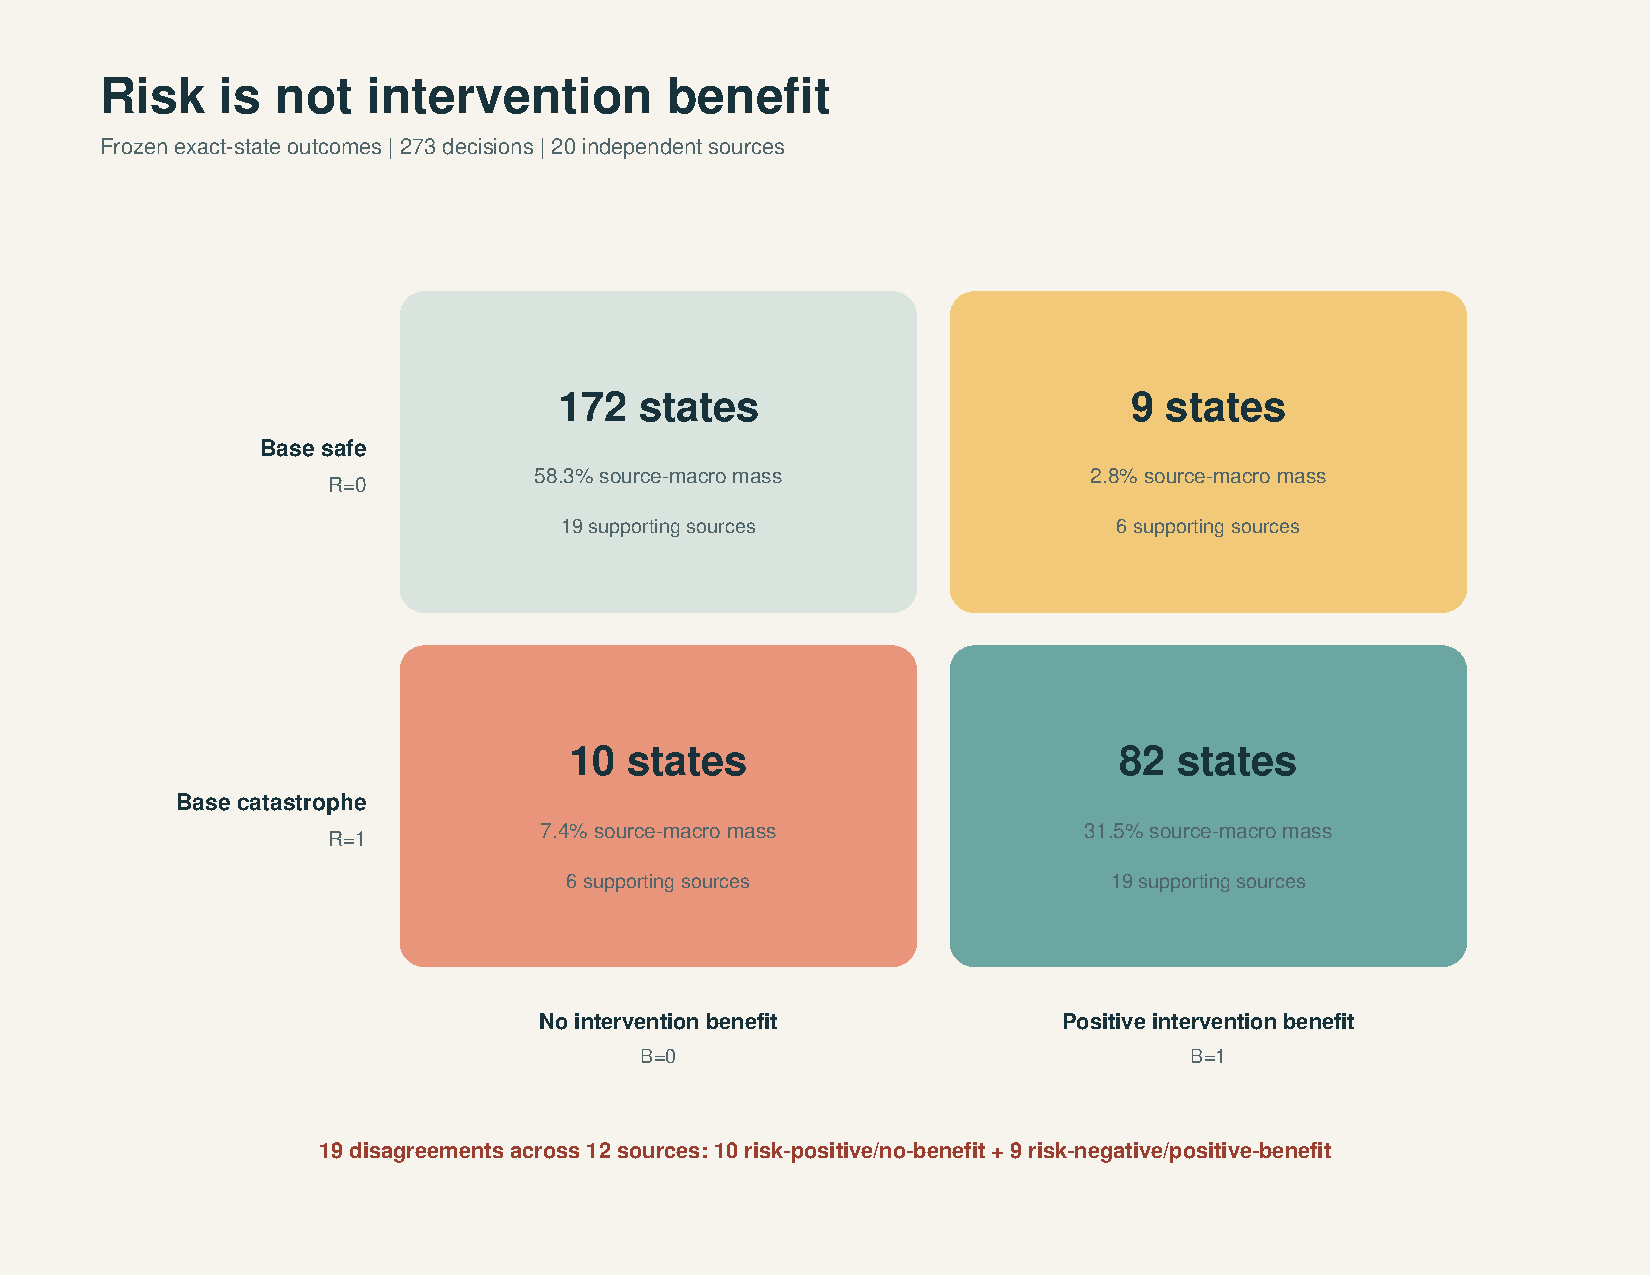
\includegraphics[width=0.94\linewidth]{figure_risk_benefit_flow.pdf}
  \caption{\textbf{Exact-state protocol and risk-benefit flow.} Top: every
  member of the finite option set begins at a hash-verified saved state; the
  privileged \Detour uses injected geometry and is not end-to-end learned.
  Bottom: the complete raw $R\times B$ table over 273 repeated decisions from
  20 independent sources. The 10 $R{=}1,B{=}0$ decisions and nine
  $R{=}0,B{=}1$ decisions each occur in six sources; their source sets are
  disjoint. All observations belong to the single \texttt{glass\_recovery}
  mechanical family.}
  \label{fig:protocol-flow}
\end{figure}

\subsection{Options, outcomes, and decision targets}

\Base continues the frozen OpenVLA policy from the restored observation.
\Detour is a privileged structured controller with access to glass geometry;
it is designed to preserve task progress and complete the original placement.
\Retreat moves back and up, then holds; it prioritizes avoiding catastrophe but
normally does not complete the task. These are fixed option contracts, not a
common action budget or a learned proposal set.

Each branch receives exactly one terminal outcome: task success, catastrophe,
or safe noncompletion, mapped to utility $+1$, $-1$, or $0$. For a saved state
$x$, let $U_B,U_D,U_R$ denote the three realized utilities. With the frozen
strict benefit epsilon of zero,
\begin{align}
  R(x) &= \mathbf{1}[Y_B=\mathrm{catastrophe}],\\
  B(x) &= \mathbf{1}[\max(U_D,U_R)>U_B],\\
  O(x) &= \arg\max_{o\in\{B,D,R\}} U_o,\\
  A_{\mathrm{int}}(x)&=\max(U_D,U_R)-U_B,\qquad
  A_{DR}(x)=U_D-U_R.
\end{align}
Oracle ties use the order \Base, \Detour, \Retreat. Strict support is a
different label: it requires a unique maximizer under the frozen support margin
$\gamma=0.5$, excluding all ties.

\subsection{Source-aware estimands}

Raw decision counts describe repeated observations. Equal-source metrics first
compute a rate within each source and then average across sources. Conditional
source-macro probabilities average only source conditionals whose denominator
is nonzero; they are not ratios of macro joint cells. Learned methods use the
frozen leave-one-source-out predictions and their existing foldwise calibration
rules. Oracle and oracle-hybrid combinations are diagnostic upper bounds, not
deployable methods.

\section{Model-Free Risk, Benefit, and Option Evidence}

\subsection{Risk and benefit disagree in both directions}

The raw $R\times B$ table contains 172 $(0,0)$, 9 $(0,1)$, 10 $(1,0)$, and 82
$(1,1)$ decisions. Thus 19/273 decisions disagree across 12 independent
sources. Ten risky Base decisions have no better intervention ($R{=}1,B{=}0$),
across six sources. Nine non-catastrophic Base decisions are nevertheless
improvable ($R{=}0,B{=}1$), also across six sources. The two source sets are
disjoint. Mechanically, the first direction is concentrated in glass (nine
glass and one offpath decision), while the second occurs only in controls (five
noglass and four offpath decisions). This supports separation within the
design, not a cross-family law.

Raw conditionals are $P(B{=}1\mid R{=}1)=82/92=0.8913$,
$P(B{=}1\mid R{=}0)=9/181=0.0497$, and
$P(R{=}1\mid B{=}1)=82/91=0.9011$. Their equal-source counterparts are
0.8700 over 20 denominator-bearing sources, 0.0415 over 19, and 0.9328 over 19.
The high association explains why risk is a strong baseline; the 19
disagreements establish only that it is not decision-complete.

\subsection{Same binary risk, different strict action}

We exhaustively form strata matched on source, condition, remaining-action
horizon, and binary $R$, retaining every stratum with at least two different
strict optimal labels. This deterministic rule yields exactly three tight
pairs across two sources (Table~\ref{tab:witnesses}); it does not select a
visually preferred subset. The only exact \Detour--\Retreat pair has one-source
support.

\begin{table}[H]
\centering
\small
\setlength{\tabcolsep}{4pt}
\begin{tabularx}{\linewidth}{@{}l l c Y Y l@{}}
\toprule
Condition & Source & $H/R$ & State A: $(B,D,R)$ & State B: $(B,D,R)$ & Strict actions \\
\midrule
glass & \texttt{69fa7e93...} & 5/1 &
\texttt{43347d99...}: (cat, success, safe) &
\texttt{f83d0199...}: (cat, cat, safe) & Detour / Retreat \\
offpath & \texttt{69fa7e93...} & 5/0 &
\texttt{db05c179...}: (success, safe, safe) &
\texttt{09da0904...}: (safe, success, safe) & Base / Detour \\
noglass & \texttt{b830bede...} & 5/0 &
\texttt{7cc66a27...}: (success, safe, safe) &
\texttt{2ccd971e...}: (safe, success, safe) & Base / Detour \\
\bottomrule
\end{tabularx}
\caption{\textbf{Complete deterministic tight-witness set.} All three pairs
are shown. They span 2 independent sources in the one
\texttt{glass\_recovery} mechanical family. The exact Detour/Retreat contrast
is supported by 1 source. ``offpath'' and ``noglass'' are controls, not
families. Full state and observation hashes plus deployable feature summaries
are in Appendix~\ref{app:witnesses}.}
\label{tab:witnesses}
\end{table}

\section{Fair Baselines and Oracle Attribution}

\subsection{The learned-method result is null}

All comparisons in this section use the same 20 source-held-out prediction
blocks and source-macro utility. \RiskBest chooses both its non-Base option and
threshold within each outer calibration fold; it is not a globally fixed
Risk-to-Detour rule. It reaches utility 0.2544. The strongest evaluated learned
method, OutcomeRouter, reaches 0.2722, a gain of only +0.0178, below the frozen
+0.03 requirement. It also misses all three strict Base/Detour/Retreat recall
requirements, so no Phase 2.5B method gate passes. The complete tiny nonlinear
advantage-decomposed router reaches 0.2311, below the risk reference, and no
advantage router passes its method gate.

The null does not erase diagnostic structure. Conditional on a true benefit
gate, the tiny nonlinear choice head passes its frozen strict Detour/Retreat
point-estimate gate, while both linear heads fail. That head is a capacity
diagnostic only: it is not the paper method, not an architecture-selection
result, and not evidence that a larger router would solve the benefit gate.

\begin{table}[H]
\centering
\small
\begin{tabularx}{\linewidth}{@{}Y r r r Y@{}}
\toprule
Policy or diagnostic & Utility & Gain vs. risk ref. & Gap to Oracle & Gate/status \\
\midrule
\RiskBest & 0.2544 & 0.0000 & 0.3097 & strong scalar-risk reference \\
OutcomeRouter & 0.2722 & +0.0178 & 0.2919 & no method pass \\
LearnedGate + OracleChoice (tiny) & 0.2714 & +0.0169 & 0.2928 & oracle diagnostic \\
OracleGate + learned linear choice & 0.4975 & +0.2431 & 0.0667 & oracle diagnostic \\
OracleGate + learned tiny choice & 0.4917 & +0.2372 & 0.0725 & capacity diagnostic \\
Full tiny ADR & 0.2311 & -0.0233 & 0.3331 & no method pass \\
\Oracle & 0.5642 & +0.3097 & 0.0000 & realized upper bound \\
\bottomrule
\end{tabularx}
\caption{\textbf{Risk reference, learned selectors, hybrids, and Oracle.}
Values are equal-source utility over 20 exposed-development sources and 273
repeated decisions. OracleGate and OracleChoice require realized labels and are
diagnostic only. No displayed learned method passes its frozen method gate.}
\label{tab:regret-main}
\end{table}

\subsection{Benefit gating dominates the reported composition gap}

The finite-option \Oracle reaches 0.5642, giving an observed opportunity of
$0.5642-0.2544=0.3097$ above \RiskBest. For the tiny candidate, OracleGate plus
learned choice loses 0.0725 from Oracle and recovers 0.7659 of that opportunity.
LearnedGate plus OracleChoice loses 0.2928 and recovers only 0.0547. The full
composition recovers $-0.0753$. In this frozen composition, benefit gating is
the dominant empirical loss. This is attribution using unavailable oracle
components, not a proposal for deployment.

\begin{figure}[H]
  \centering
  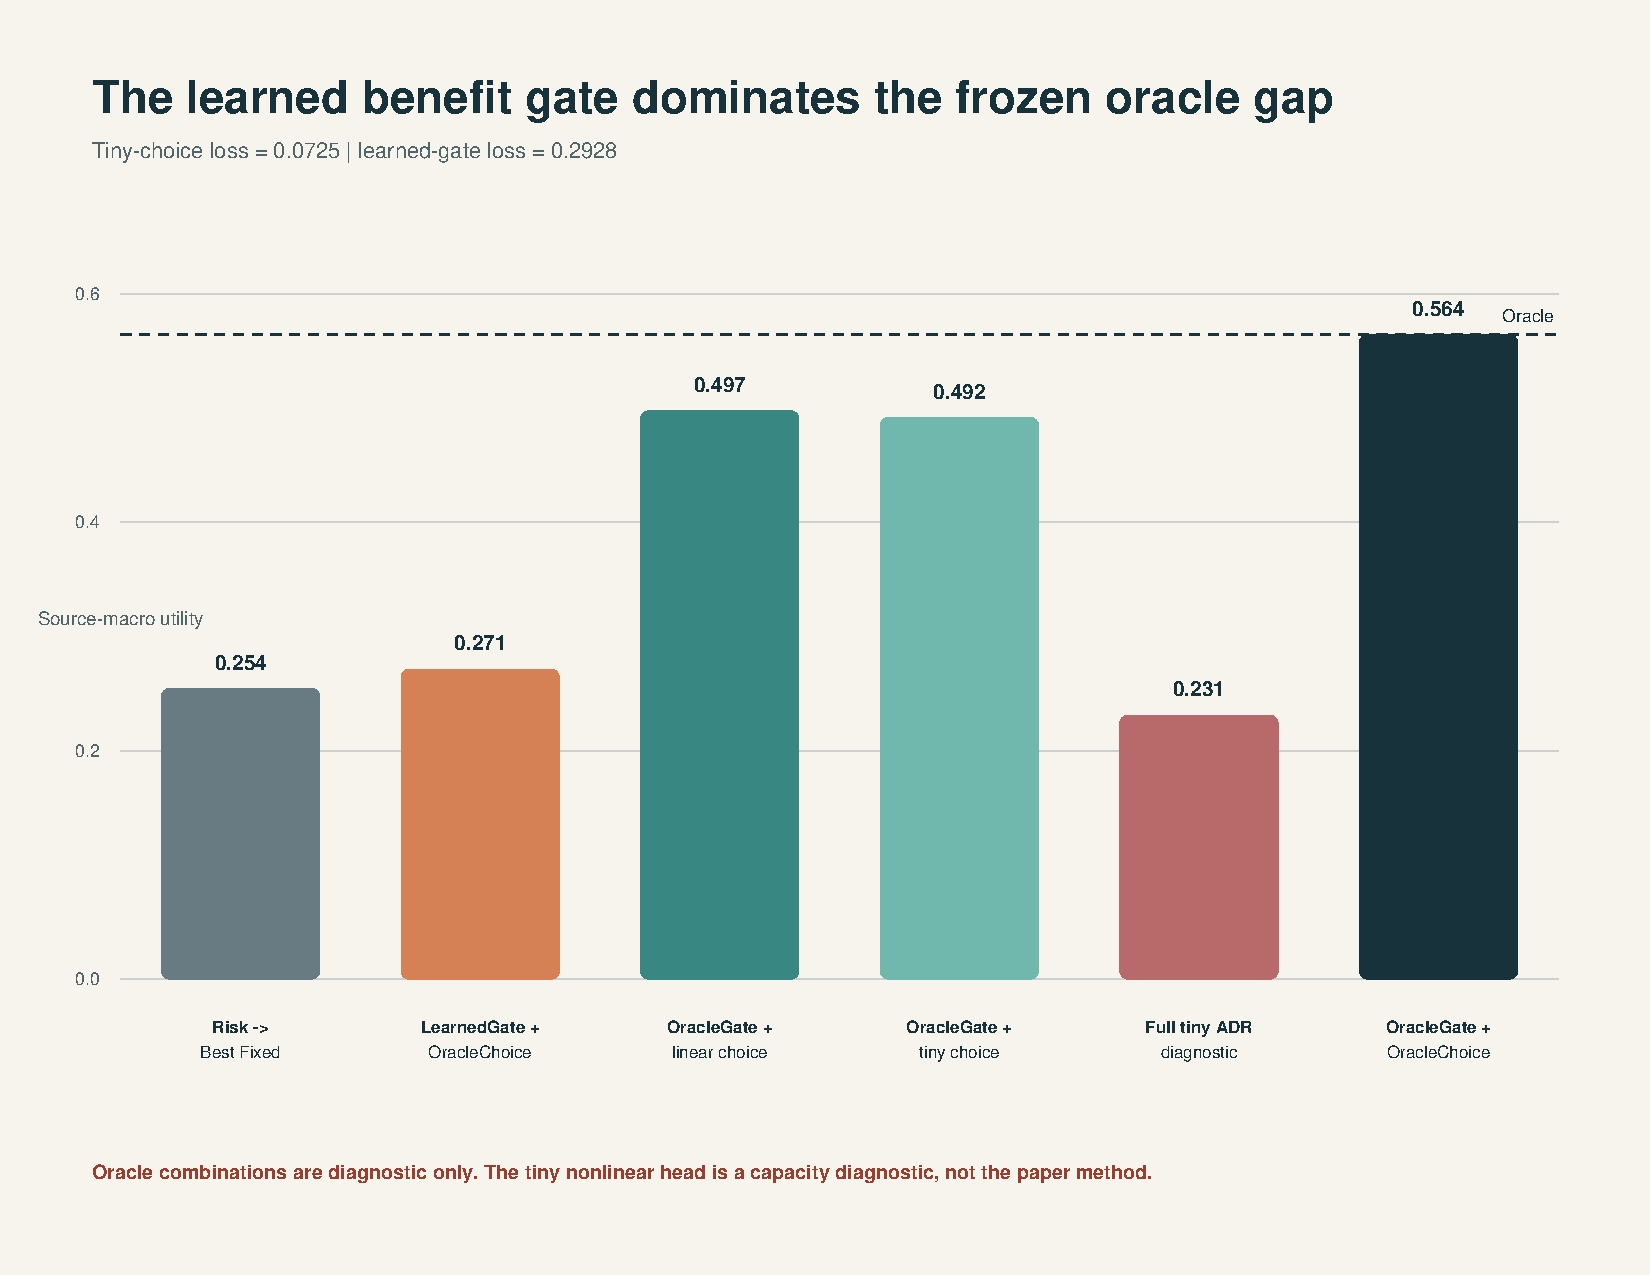
\includegraphics[width=0.96\linewidth]{figure_oracle_gap_waterfall.pdf}
  \caption{\textbf{Oracle-gap attribution.} Source-macro utilities use the
  same 20 exposed-development sources. The 0.3097 opportunity is the observed
  difference between \RiskBest (0.2544) and the realized finite-option Oracle
  (0.5642). Every OracleGate or OracleChoice bar is diagnostic only. The tiny
  nonlinear head is a conditional capacity diagnostic, not a successful
  router.}
  \label{fig:oracle-gap}
\end{figure}

\section{Source and Mechanical-Scope Audit}

Nineteen of 20 sources contain both benefit labels. Strict support is present
for Base, Detour, and Retreat in 16, 13, and 9 sources, respectively. However,
pooled source counts conceal mechanical concentration. Glass contains 101
decisions from 20 sources, offpath 86 from 17, and noglass 86 from 17. All 23
strict Retreat states, across nine sources, are glass. Glass also contains
51/60 strict Detour-or-Retreat states across 16 sources; all 60 occur across 17
sources. Non-glass controls contribute nine strict Detour states across six
sources and no strict Retreat state.

Five sources contain both a strict Detour and a strict Retreat label when
conditions are pooled, but only two contain such a flip within glass. The
tight exact Detour/Retreat witness in Table~\ref{tab:witnesses} has one source.
These nested counts are not interchangeable. They support a glass-scoped
diagnosis while ruling out a claim of broad option ambiguity.

\begin{figure}[H]
  \centering
  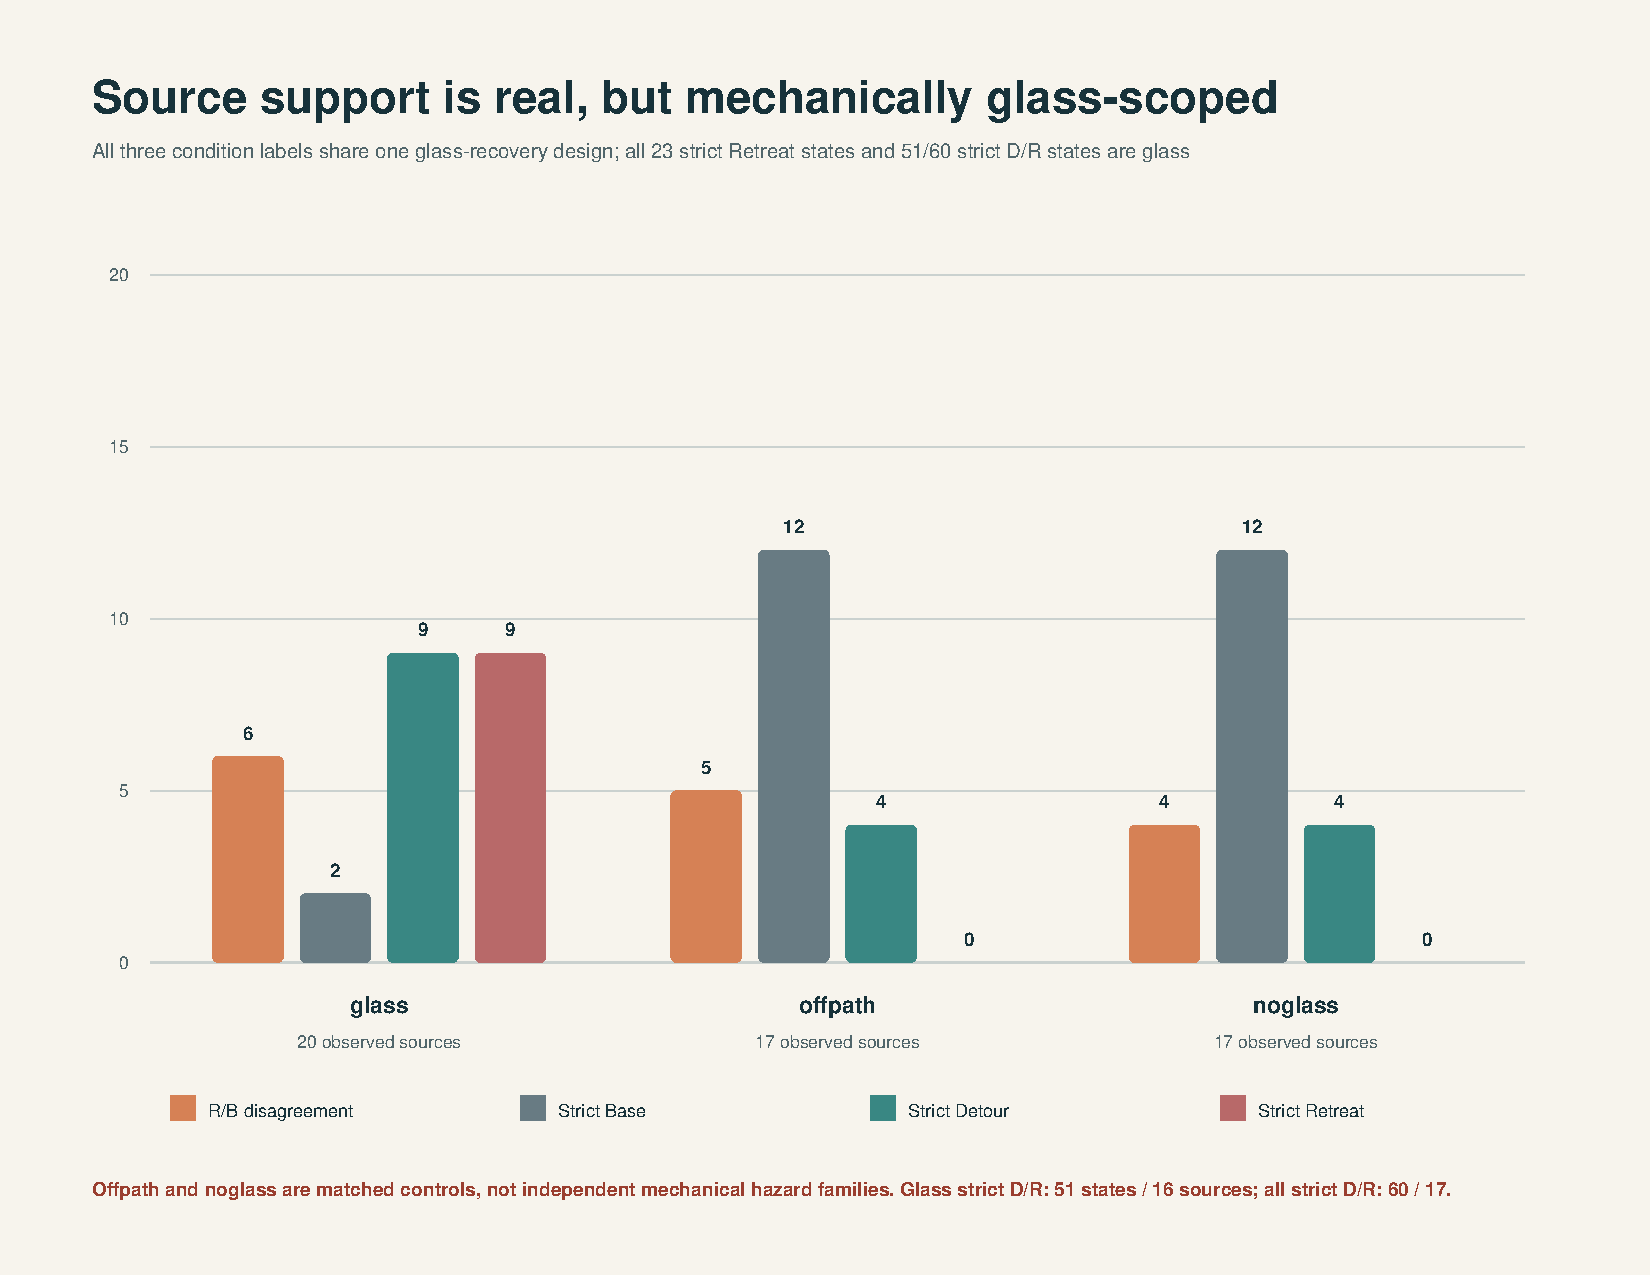
\includegraphics[width=0.96\linewidth]{figure_source_support.pdf}
  \caption{\textbf{Condition-level source support within one mechanical
  family.} The 20-source universe has condition-specific effective counts of
  20/17/17 sources for glass/offpath/noglass, respectively. The bars show
  effective independent-source counts separately for
  the \texttt{glass}, \texttt{offpath}, and \texttt{noglass} conditions.
  All conditions share the single \texttt{glass\_recovery} family; offpath and
  noglass are matched controls. Glass supplies all 23 strict Retreat states
  (nine sources) and 51/60 strict Detour-or-Retreat states (16 of the 17
  sources supporting any strict D/R state).}
  \label{fig:source-scope}
\end{figure}

\section{From Statewise Opportunity to Sequential Realization}

Statewise exact branching gives labels at authored states. A sequential policy
must reach those states from reset and cross a decision boundary at a useful
time without unnecessary control interventions. The frozen sequence in
Table~\ref{tab:sequential} is therefore a boundary analysis, not a second
method arc.

Matched-state source-OOF evaluation contains a large Oracle opportunity, yet
OutcomeRouter gains only +0.0178 and no method passes. On four development
sources, P2 changes 7/12 successes and 4/12 catastrophes to 8/12 and 3/12 at
2/12 interventions, while missing both known T-20 recoveries. Simple temporal
summaries in P2.5 do not repair the ordering. P3.1 then obtains extremely high
offline source-held-out separation (AUC 1.000 for recovery-open versus hard
control and 0.995 for intervention-needed versus hard control), but only 0.632
source-macro accuracy.

The decisive fresh P3.2 closeout uses eight sources and three conditions per
source. The direct selector chooses \Base in all 24 episodes. It therefore has
zero false interventions by inactivity, not by successful selectivity. It
recovers 0/8 glass episodes and misses 2/2 known recovery opportunities. The
older P2 comparator selects Detour in 5/24, recovers 1/8 glass episodes, and
retains 16/16 control successes. Neither result authorizes reliable sequential
intervention, and the frozen threshold is not reopened.

\begin{table}[H]
\centering
\small
\begin{tabularx}{\linewidth}{@{}l Y r Y@{}}
\toprule
Stage & Evidence & Sources/units & Scoped interpretation \\
\midrule
Matched state & Oracle 0.5642; risk ref. 0.2544; OutcomeRouter 0.2722 & 20/273 & opportunity exists; learned gain +0.0178; no pass \\
P2 & 7/12 to 8/12 success; 4/12 to 3/12 catastrophe; 2/12 intervention & 4/12 & development only; misses 2/2 known recoveries \\
P2.5 & raw max AUC 0.357; MA-3/5/8 AUC 0.286 & 4/11 & tested simple temporal summaries do not repair ordering \\
P3.1 & recovery-open AUC 1.000; intervention-needed AUC 0.995; accuracy 0.632 & 9/142 & offline source-held-out separability only \\
P3.2 & Direct: Base 24/24; glass recovery 0/8; known misses 2/2 & 8/24 & fresh first-crossing collapse to Base \\
\bottomrule
\end{tabularx}
\caption{\textbf{Statewise-to-sequential evidence.} The fresh closeout has 8
sources. Sources are independent;
units are repeated decisions, anchors, or episodes as indicated. The P3.2
negative closeout is one fresh eight-source cohort in the same
\texttt{glass\_recovery} design, not evidence that all sequential methods are
impossible.}
\label{tab:sequential}
\end{table}

\section{Limitations and Safety Scope}

\paragraph{Scope and statistical unit.}
This is one frozen OpenVLA checkpoint, one LIBERO task, one embodiment, and one
glass-recovery mechanical design. All 20 sources are exposed development.
Decision counts are repeated observations; source counts are the inferential
unit. The three condition labels are not independent hazard families. Exact
Detour/Retreat ambiguity has only one-source support.

\paragraph{Options and utility.}
The result is conditional on exactly three engineered options and the frozen
$+1/0/-1$ utility. Privileged Detour uses geometry unavailable to a generic
deployment. Retreat is a conservative safe-abort controller rather than a task
recovery policy. The utility does not charge different duration, path length,
latency, or control effort, so Oracle is only the best realized option under
this contract.

\paragraph{Restoration and artifact availability.}
The collector verifies five branch-start hashes, but does not record a separate
per-decision global RNG-state hash. Deterministic decoding and fixed seed limit
the practical dependence without proving byte-identical RNG restoration. Raw
capture files are locally hash-pinned but ignored by Git; the reviewed PIVOT
tables, figures, and manifests are tracked. Raw witness pixels were not
retained, so the released witness table provides observation hashes and feature
summaries rather than images.

\paragraph{Learning and sequential deployment.}
No learned method passes the frozen method gate. The tiny nonlinear choice
result is conditional on an oracle gate. High offline P3.1 AUC does not transfer
to fresh first crossing. The P3.2 null closes this protocol, not every possible
temporal model. We do not propose threshold lowering, another router, or a new
cohort from these results.

\paragraph{Ethics and safety.}
All claim-bearing outcomes are simulated robot manipulation; no human-subject
or personal data are used. The diagnostic could help expose unsafe assumptions
in runtime intervention systems, but it is not a safety certificate. Reporting
the null method and sequential results reduces the risk that an offline oracle
gap is mistaken for deployable protection. Any real-robot use would require
independent mechanical validation, calibrated monitoring, fail-safe hardware,
and task-specific oversight beyond this study.

\section{Conclusion}

Within one frozen OpenVLA--LIBERO glass-recovery design, realized exact-state
outcomes show that Base catastrophe status does not uniquely determine
intervention benefit or the best finite option. The phenomenon is supported by
12 sources for risk-benefit disagreement but by only two sources for tight
same-risk action pairs, with one source for the exact Detour/Retreat witness.
A substantial observed Oracle opportunity remains, yet the evaluated learned
selectors do not pass their method gates and the fresh sequential selector
collapses to Base. The defensible result is a source-aware, glass-scoped
diagnostic and negative-result case study. Broader claims require separately
authorized evidence across mechanical families, tasks, policies, and
confirmatory sources; they are not inferred here.

\bibliographystyle{plainnat}
\bibliography{references}

\clearpage
\appendix
\section{Frozen Corpus and Provenance}
\label{app:provenance}

Table~\ref{tab:provenance} records the contracts used by every main-text
number. The PIVOT-0 synthesis generated no rollout and trained no model; it
reads frozen Phase 2.5A, Phase 2.5B, Phase 2.5B-R, and sequential-closeout
artifacts. Historical train/calibration/development names remain provenance
fields only. PIVOT-0 treats all 20 sources as exposed development.

\begin{table}[H]
\centering
\small
\begin{tabularx}{\linewidth}{@{}l Y@{}}
\toprule
Contract & Frozen value \\
\midrule
Policy checkpoint & \texttt{openvla/openvla-7b-finetuned-libero-spatial}, revision \texttt{962318cec55ac10993ff0f5f43eda9a270b4c873} \\
Capture commit & \texttt{d4751330395eec11691f4830761b76f5f1ac36b7} (clean) \\
Capture protocol hash & \texttt{b487d8b5cc20c1fe932d8ee4ff67f05883e2b010b6ee9eb155eb9b93c2d1a4c3} \\
PIVOT generation commit & \texttt{98b3ffe0aec2838448d0536b6c62036e37487f6f} (clean) \\
PIVOT evidence fingerprint & \texttt{dc48ff317dad}; capture fingerprint \texttt{d4751330395e} \\
Sources and decisions & 20 exposed-development sources; 273 eligible decisions; 819 realized option rows \\
Historical split provenance & 5 train, 7 calibration, 8 development sources; no confirmatory split in this synthesis \\
Mechanical scope & one \texttt{glass\_recovery} family; \texttt{glass} treatment plus \texttt{offpath}/\texttt{noglass} controls \\
Options & \texttt{base\_continue}, privileged \texttt{detour\_complete}, \texttt{retreat\_hold} \\
Outcomes and utility & task success $=+1$; safe noncompletion $=0$; catastrophe $=-1$ \\
Decode and seed & deterministic decoding (no sampling, one beam); rollout seed 0 \\
PIVOT actions & new rollouts false; new training false; fresh test outcomes loaded false \\
\bottomrule
\end{tabularx}
\caption{Frozen corpus and provenance contract. Effective independent sources:
20; repeated decisions: 273.}
\label{tab:provenance}
\end{table}

\section{Exact Restoration, Eligibility, and Finite-Option Semantics}
\label{app:restore}

\paragraph{Saved state.}
The collector stores flattened MuJoCo time, $qpos$, and $qvel$; exact model XML;
OSC goals, gains, torques, and interpolator state; integration inputs; episode
counters; robot temporal buffers; observable values and timers; the observation
cache; and the explicit policy-boundary observation. The historical name
``controller state'' therefore denotes a broader continuation snapshot, not
only an OSC command.

\paragraph{Five required identities.}
Before each option branch, the collector rebuilds the model, restores the
numeric state and continuation snapshot, and recomputes SHA-256 identities for
(i) simulator state, (ii) controller/dynamics state excluding scene-specific
observations, (iii) the complete numeric continuation including observation
history, (iv) every policy-boundary observation field with dtype and shape, and
(v) model XML. Any mismatch raises \texttt{exact\_state\_restore\_mismatch} and
the decision cannot be retained. The 273 retained decisions each have three
completed option rows under this fail-closed code path.

\paragraph{RNG boundary.}
The run fixes seed 0 and deterministic policy generation, and the structured
controllers are deterministic. The stored branch identities do not include a
separate serialization or hash of global Python, NumPy, or framework RNG state
at every decision. The exact-state claim in this paper is restricted to the
five verified branch-start identities. A broader benchmark should add explicit
RNG serialization even when decoding is deterministic.

\paragraph{Eligibility.}
Source/placement eligibility is mechanical and Base-defined, not selected by a
router result. Exclusions include invalid initial catastrophe, on-path failure
to produce the intended catastrophe, catastrophe before the requested horizon,
and a control terminating before the matched anchor. A placement/condition/
horizon enters only when a valid branch start exists. All retained branches
receive exactly one of the three terminal outcomes. The PIVOT synthesis keeps
all 273 retained decisions and does not recensor after observing option labels.

\paragraph{Interpretation.}
Executing all three branches is full information for this finite option set at
these saved states. It does not identify the value of an unexecuted controller,
an observational population effect, or the best policy in a continuous action
space. Privileged Detour receives obstacle geometry. Retreat is a conservative
fallback. Their different control horizons and effort are not charged by the
frozen utility.

\section{Complete Risk-Benefit Accounting}
\label{app:risk-benefit}

\begin{table}[H]
\centering
\small
\begin{tabular}{@{}lrrr@{}}
\toprule
Cell & Raw decisions & Supporting sources & Equal-source joint mass \\
\midrule
$R=0,B=0$ & 172 & 19 & 0.5831 \\
$R=0,B=1$ & 9 & 6 & 0.0278 \\
$R=1,B=0$ & 10 & 6 & 0.0742 \\
$R=1,B=1$ & 82 & 19 & 0.3150 \\
\midrule
Total & 273 & 20 & 1.0000 \\
\bottomrule
\end{tabular}
\caption{Raw and equal-source $R\times B$ accounting over 20 independent
sources. A supporting-source
count means that the source contains at least one decision in the cell; counts
therefore do not sum to 20.}
\label{tab:rb-full}
\end{table}

The raw conditional probabilities are 0.8913 for $P(B=1\mid R=1)$, 0.0497 for
$P(B=1\mid R=0)$, and 0.9011 for $P(R=1\mid B=1)$. Equal-source conditional
means are respectively 0.8700 over 20 denominator-bearing sources, 0.0415 over
19, and 0.9328 over 19. Ratios of the equal-source joint cells in
Table~\ref{tab:rb-full} are different estimands and are not substituted for
these conditional means.

The 10 $R=1,B=0$ decisions occur at horizons 5/10/30/40 in counts 6/1/1/2 and
conditions glass/offpath in counts 9/1. The nine $R=0,B=1$ decisions occur at
horizons 5/10/20/30 in counts 5/2/1/1 and conditions noglass/offpath in counts
5/4. Each direction has six sources, and the source sets are disjoint.

\section{Complete Tight Witnesses}
\label{app:witnesses}

The deterministic witness rule matches source, condition, horizon, and binary
risk exactly. Table~\ref{tab:witness-detail} contains every resulting pair.
The ``feature summary'' columns are computed from deployable robot state,
nominal action, and frozen hidden features. Raw pixels are not retained; exact
observation and hidden hashes make that limitation explicit.

\small
\begin{longtable}{@{}p{0.16\linewidth}p{0.79\linewidth}@{}}
\caption{Full deterministic witness records: 3 pairs across 2 independent
sources, with 1 source for the exact Detour/Retreat contrast.}\label{tab:witness-detail}\\
\toprule
Field & Value \\
\midrule
\endfirsthead
\toprule
Field & Value \\
\midrule
\endhead
Pair 1 stratum & mechanical family \texttt{glass\_recovery}; condition \texttt{glass}; source \nolinkurl{69fa7e93588c6aea4b134efa44633d38556ce1656b46df276021920a664881a3}; $H=5$; $R=1$ \\
Pair 1 states & A \nolinkurl{43347d99e35479cdc3d3197e5c6127d8bb063ec834656eecdd505a39f52d7167}; B \nolinkurl{f83d0199d1f4fdc40ae28dc3a5c02514dc5ae737d391602dea012bb750f98642} \\
Pair 1 observations & A \nolinkurl{fe26c03740a7719695c9e5e2bdbac19a64e0bcb93c52ce587fb187c95f55652e}; B \nolinkurl{cd048daaae15635b63b6ea1c4568163ee75066ca3ae1eccb7cb69c2323750e64} \\
Pair 1 outcomes/utility & A: (Base catastrophe $-1$, Detour success $+1$, Retreat safe $0$), strict Detour. B: (Base catastrophe $-1$, Detour catastrophe $-1$, Retreat safe $0$), strict Retreat. \\
Pair 1 feature summary & z-scored robot/action distance 3.2781; hidden cosine distance 0.6481; hidden hashes A \nolinkurl{9810a1fd95eb8fb0b82787c1f52adf76c98e2f27c1683fa32b238eb2c60955ad}, B \nolinkurl{334985f6df5e8d698a1d0e06d3a8ddbb9c04d556257be6a8f5d33c7b2bb94de3}. \\
\midrule
Pair 2 stratum & mechanical family \texttt{glass\_recovery}; condition \texttt{offpath}; source \nolinkurl{69fa7e93588c6aea4b134efa44633d38556ce1656b46df276021920a664881a3}; $H=5$; $R=0$ \\
Pair 2 states & A \nolinkurl{db05c17974a1032f5835681f51f63fcb978004eecfe48098e0892f5bd6ada082}; B \nolinkurl{09da0904e292712e5ed0fbdeaeb877e637acabfb5f929d8276f5fdb0c3004a96} \\
Pair 2 observations & A \nolinkurl{226d3ac32a8c77573e890d4948eb07e0ffd911eddb26ee53763ae5ab885734b7}; B \nolinkurl{910cb06477e5969823bbb792a43446d4c99146799c761208495a74730aabf11a} \\
Pair 2 outcomes/utility & A: (Base success $+1$, Detour safe $0$, Retreat safe $0$), strict Base. B: (Base safe $0$, Detour success $+1$, Retreat safe $0$), strict Detour. \\
Pair 2 feature summary & z-scored robot/action distance 3.8686; hidden cosine distance 0.4464; hidden hashes A \nolinkurl{4c1b430253f5e6f64a19ea060abb815b8ffa91a1e675b1649466d6b0c2832f35}, B \nolinkurl{5a148ac7f5e7145c671ab2eb0996613473be787531dc17889ecacc5d1a8a617e}. \\
\midrule
Pair 3 stratum & mechanical family \texttt{glass\_recovery}; condition \texttt{noglass}; source \nolinkurl{b830bede73f505b84b88a6596e92c22a5a4c0ded1e275e8e5b28a599849d2df6}; $H=5$; $R=0$ \\
Pair 3 states & A \nolinkurl{7cc66a27ce2971b4dd170aa8f8b415751cf10acaf0a4eb4a2ac10682c2b9dda6}; B \nolinkurl{2ccd971e77ce745c2eb16199826277fcd3c3072243e5e2d9b5214fb4b1d0b89c} \\
Pair 3 observations & A \nolinkurl{44fadc36ca73e1c03ec22f5653aed6748c82f7bc39c7ce1edfc8fc4c7813faa1}; B \nolinkurl{7dd048488f8e3683036bd9e47426b4b98b05ffb109f09eaa99d814ccca3f07fa} \\
Pair 3 outcomes/utility & A: (Base success $+1$, Detour safe $0$, Retreat safe $0$), strict Base. B: (Base safe $0$, Detour success $+1$, Retreat safe $0$), strict Detour. \\
Pair 3 feature summary & z-scored robot/action distance 2.0406; hidden cosine distance 0.6742; hidden hashes A \nolinkurl{c9370f4f86e582a51e3fc1acc5023bf8854e57817c7196dca65773a31a98ae85}, B \nolinkurl{97d05dc72f018a054679495cfd8d7584f80389153a74862f086099ce9ec99c26}. \\
\bottomrule
\end{longtable}
\normalsize

Pair 1 is the only exact Detour/Retreat contrast and has one independent
source. Pairs 1 and 2 share that source, so the complete three-pair set has two
independent sources, not three.

\section{Complete Source-Macro Policy-Regret Table}
\label{app:policy-regret}

\begin{table}[H]
\centering
\scriptsize
\setlength{\tabcolsep}{3.5pt}
\begin{tabular}{@{}lrrrrrrr@{}}
\toprule
Policy & Success & Cat. & Safe & Interv. & Utility & Regret & Opp. rec. \\
\midrule
Always Base & .5197 & .3892 & .0911 & .0000 & .1306 & .4336 & -.4000 \\
Always Detour & .4347 & .1800 & .3853 & 1.0000 & .2547 & .3094 & .0009 \\
Always Retreat & .0000 & .1858 & .8142 & 1.0000 & -.1858 & .7500 & -1.4215 \\
Risk $\rightarrow$ Detour & .4989 & .2511 & .2500 & .4981 & .2478 & .3164 & -.0215 \\
Risk $\rightarrow$ Retreat & .4394 & .3097 & .2508 & .3506 & .1297 & .4344 & -.4027 \\
Risk $\rightarrow$ Best Fixed & .5022 & .2478 & .2500 & .4947 & .2544 & .3097 & .0000 \\
Oracle Benefit Gate $\rightarrow$ fixed Detour & .6383 & .1483 & .2133 & .3428 & .4900 & .0742 & .7605 \\
OracleGate + tiny learned choice & .6158 & .1242 & .2600 & .3428 & .4917 & .0725 & .7659 \\
Tiny LearnedGate + OracleChoice & .4878 & .2164 & .2958 & .4567 & .2714 & .2928 & .0547 \\
Full tiny ADR & .4733 & .2422 & .2844 & .4567 & .2311 & .3331 & -.0753 \\
Oracle & .6383 & .0742 & .2875 & .3428 & .5642 & .0000 & 1.0000 \\
\bottomrule
\end{tabular}
\caption{All policy-regret rows under the same 20 sources and 273 repeated
decisions under the
source-macro contract. ``Opp. rec.'' is the fraction of the Oracle improvement
above Risk $\rightarrow$ Best Fixed. Negative values mean a policy falls below
that risk reference. Oracle gates/choices are diagnostic and unavailable at
deployment.}
\label{tab:policy-full}
\end{table}

The Phase 2.5B OutcomeRouter row is not repeated in
Table~\ref{tab:policy-full} because the frozen PIVOT policy-regret CSV records
the fixed/risk/oracle-hybrid composition table. Under the same 20 source blocks,
OutcomeRouter has success 0.5008, catastrophe 0.2286, intervention 0.4831, and
utility 0.2722. Its +0.0178 utility gain over the 0.2544 risk reference is below
the +0.03 gate and it fails the three strict-recall criteria.

\section{Learned Selector and Attribution Audits}
\label{app:learned}

\begin{table}[H]
\centering
\small
\begin{tabular}{@{}lrrrrl@{}}
\toprule
Method & Utility & Base rec. & Detour rec. & Retreat rec. & Frozen result \\
\midrule
Risk $\rightarrow$ Best Fixed & .2544 & .5595 & .5705 & .0556 & reference \\
OutcomeRouter & .2722 & .5926 & .3269 & .3704 & no pass \\
Support-balanced OutcomeRouter & .2672 & .6534 & .3013 & .4815 & no pass \\
Hidden-only OutcomeRouter & .2644 & .4881 & .4359 & .5185 & no pass \\
ADR linear full & .2097 & .5874 & .3910 & .2593 & no pass \\
ADR linear split & .2222 & .4999 & .4487 & .3704 & no pass \\
ADR tiny nonlinear choice & .2311 & .5749 & .4551 & .4444 & no pass \\
\bottomrule
\end{tabular}
\caption{Frozen source-OOF learned-selector results over 20 sources. Phase 2.5B is
\texttt{INCONCLUSIVE} and fail-closed; Phase 2.5B-R records
\texttt{CHOICE\_CAPACITY\_BOTTLENECK} while every complete ADR has
\texttt{method\_pass=false}.}
\label{tab:method-null}
\end{table}

On the 60 strict Detour/Retreat decisions, conditional balanced accuracy is
0.5579 for the full linear head, 0.6369 for the split linear head, and 0.7253
for the fixed tiny nonlinear head. Their Detour/Retreat recalls are
0.7421/0.3738, 0.8354/0.4385, and 0.8559/0.5947. Only the tiny conditional head
passes the point-estimate choice gate. All candidates share a weak learned
benefit score (AUROC 0.6062, AUPRC 0.4783), and no full composition passes.

For the tiny candidate, the source-macro losses from Oracle are 0.0725 for
OracleGate plus learned choice, 0.2928 for LearnedGate plus OracleChoice, and
0.3331 for the full composition. The split-linear OracleGate hybrid reaches
0.4975, slightly above the tiny hybrid's 0.4917. The tiny head is therefore not
selected as a generally superior model; it diagnoses conditional capacity only.

\section{Condition and Horizon Support}
\label{app:support}

\begin{table}[H]
\centering
\small
\begin{tabular}{@{}lrrrrrrrr@{}}
\toprule
Condition & Decisions & Sources & $R\ne B$ & $R\ne B$ src. & Strict B & Strict D & Strict R & D/R ties \\
\midrule
glass & 101 & 20 & 9 & 6 & 2 & 28 & 23 & 31 \\
offpath & 86 & 17 & 5 & 5 & 24 & 4 & 0 & 0 \\
noglass & 86 & 17 & 5 & 4 & 35 & 5 & 0 & 0 \\
\bottomrule
\end{tabular}
\caption{Condition accounting over a 20-source universe inside the single
\texttt{glass\_recovery} mechanical family; glass/offpath/noglass contribute
20/17/17 sources. Here B/D/R in the strict columns denote Base, Detour, and
Retreat, not the binary benefit variable.}
\label{tab:condition-support}
\end{table}

Across all conditions, strict Base/Detour/Retreat counts are 61/37/23 and their
source supports are 16/13/9. Horizon-level strict Base/Detour/Retreat counts are
4/2/1 at H40, 15/6/1 at H30, 16/8/5 at H20, 11/11/9 at H10, and 15/10/7 at H5.
Retreat support is both glass-only and late-state concentrated: 16/23 strict
Retreat decisions occur at H5 or H10.

Nineteen sources contain both benefit labels. Nine contain a strict Base/Detour
flip, nine a strict Base/Retreat flip, and five a pooled strict Detour/Retreat
flip. Only two have a within-glass strict Detour/Retreat flip. The complete
per-source flag matrix is the tracked \texttt{source\_support.csv}; it is not
expanded into 20 rows here because the artifact map identifies the exact file
and SHA-256.

\section{Expanded Sequential Boundary}
\label{app:sequential}

\begin{table}[H]
\centering
\scriptsize
\begin{tabularx}{\linewidth}{@{}l l r r r r Y@{}}
\toprule
Stage & Method/diagnostic & Sources & Units & Success & Interv. & Frozen reading \\
\midrule
P2 & exact T-20 opportunity & 4 & 4 & 2 known & -- & option label, not policy \\
P2 & fixed T-20 Router & 4 & 12 & 7/12 & 0/12 & misses 2/2 known opportunities \\
P2 & dynamic first crossing & 4 & 12 & 8/12 & 2/12 & 3/12 catastrophes; development only \\
P2.5 & trajectory morphology & 4 & 11 & -- & -- & raw max AUC .357; moving-average AUC .286 \\
P3.1 & direct head strict LOSO & 9 & 142 & -- & -- & recovery AUC 1.000; needed AUC .995; source-macro accuracy .632 \\
P3.2 & old P2 comparator & 8 & 24 & 17/24 & 5/24 & recovers 1/8 glass; two unnecessary control interventions \\
P3.2 & direct recovery Router & 8 & 24 & 16/24 & 0/24 & Base 24/24; recovers 0/8 glass; misses 2/2 \\
P3.2 & exact T-20 Detour & 8 & 8 & 2/8 & -- & option diagnostic; not deployed timing \\
P3.2 & trajectory maxima & 2 positive & 24 & -- & 0/24 & known-recovery vs control AUC .250 \\
\bottomrule
\end{tabularx}
\caption{Complete frozen statewise-to-sequential summary over stage-specific
sets of 4, 9, and 8 sources. ``Units'' are
repeated decisions, anchors, or episodes, not additional independent sources.}
\label{tab:sequential-full}
\end{table}

The direct P3.2 method's zero false interventions are mechanically coupled to
choosing Base in every episode. They are not evidence of a selective policy
that both preserves controls and intervenes on opportunities. The old P2
comparator retains task success on all 16 controls but recovers only one of
eight glass episodes. These results close threshold and temporal rescue for the
frozen protocol; they do not prove that sequential intervention is impossible.

\section{Artifact Availability and Reproduction Boundary}
\label{app:availability}

The reviewed PIVOT manifest, seven CSV tables, story decision, and three PDF
figures are tracked in Git and hash-pinned by the PIVOT manifest. The capture
manifest, feature archive, decision metadata, and option-rollout JSONL are
present in the working environment and match the hashes recorded by PIVOT, but
the \texttt{results/counterfactual\_router/} directory is ignored by Git. A
clean repository checkout therefore supports auditing all paper numbers from
tracked reviewed summaries, but does not by itself contain the raw hidden
features or 819 branch rows. We call this
\texttt{local\_untracked\_hash\_pinned}, not repository-tracked availability.

The root ICLR manifest predates PIVOT-0 and does not enumerate the later PIVOT
package. We preserve that frozen manifest and add the publication artifact map
instead of rewriting history. The PIVOT manifest pins its outputs but cannot
self-pin its own bytes; the publication artifact map records the current
manifest hash separately. Generation commits and later record commits are kept
as distinct fields.

The local package audit verifies PIVOT required-artifact membership and hashes,
all headline values, source/family language, prohibited affirmative claims,
artifact-map schema, PDF existence, and the absence of unfinished markers.
Repository audit and unit tests remain separate checks. None of these commands
opens a simulator, fits a model, or contacts Quest.

\section{Non-Glass v1 Exclusion}
\label{app:nonglass}

The optional unstable-placement v1 job is not scientific evidence for this
paper. It attempted eight nominal source candidates, marked two as selected
before location resolution, resolved zero physical blocks, opened zero option
decisions, performed zero restoration audits, and produced zero ordinary
option-outcome rows. Its terminal status is
\texttt{INVALID\_PREFLIGHT\_ZERO\_OPTION\_OUTCOMES}. The failure was an
engineering geometry/source-freeze defect, not a positive or negative result
about non-glass intervention ambiguity. v1 contributes nothing to the 20-source
or 273-decision denominators and is mentioned here only to make exclusion
auditable.

\section{Claim Boundary Checklist}
\label{app:claims}

\begin{table}[H]
\centering
\small
\begin{tabularx}{\linewidth}{@{}Y Y@{}}
\toprule
Supported within scope & Not established \\
\midrule
Exact realized outcomes distinguish Base risk, intervention benefit, best
finite option, and sequential realization in one frozen design. & A universal
theorem about risk, regret, hazards, tasks, backbones, or controllers. \\
Risk and benefit disagree on 19/273 decisions across 12 sources. & A broad,
confirmatory VLA-safety benchmark. \\
Three exact tight pairs occur across two sources; the D/R witness has one
source. & Reliable non-glass Retreat support or replicated cross-mechanism
option ambiguity. \\
Risk $\rightarrow$ Best Fixed leaves an observed 0.3097 finite-option Oracle
opportunity. & A reachable or learned Oracle at deployment. \\
Benefit gating dominates the reported oracle-hybrid loss. & A successful,
superior, or deployable learned router. \\
Fresh direct first crossing collapses to Base in this protocol. & The
impossibility of all temporal or sequential intervention methods. \\
\bottomrule
\end{tabularx}
\caption{Submission-facing claim boundary. The core corpus has 20 sources; the
tight witness set has 2 sources and its exact Detour/Retreat contrast has 1.}
\label{tab:claim-boundary}
\end{table}


\end{document}
